\documentclass{article}
\usepackage{graphicx} % Required for inserting images
\usepackage{geometry}
\usepackage{amsmath}
\usepackage{listings}
\usepackage{hyperref}

\title{Analisis y Diseño de Algoritmos}
\author{Marco Antonio Bastida Flores}
\date{20 Junio 2023}

\geometry{left = 30mm, right = 25mm, top = 30mm, bottom = 20mm}

%------------------------------------------------------------------------%

\begin{document}

\maketitle

\section{Depth-first search}

\vspace{5mm} %5mm vertical space

%\begin{lstlisting}[language=Python]
\lstinputlisting[language=Python]{DFS.py}
%\end{lstlisting}

\vspace{5mm} %5mm vertical space

Se presenta arriba el codigo para el algoritmo de busqueda a profundidad, se hace uso de una lista ligada simple utilizando un diccionario de Python, que contiene como "key" el nodo y como "values" los nodos a los que apunta. 
Se selecciona un nodo aleatoriamente entre los elementos de los nodos para obtener el primer grafo no convexo. 
Con los nodos restantes se selecciona otro nodo aleatoriamente y se obtiene el segundo grafo no convexo. 

\vspace{5mm} %5mm vertical space

\subsection{Resultados}

En la siguiente figura se muestran los resultados

\begin{figure}[ht]
    \centering
    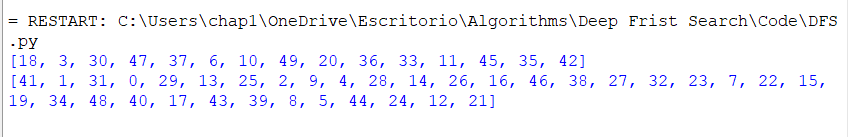
\includegraphics[scale=0.85]{results_dfs.png}
    \caption{Resultados de busqueda por profundidad}
    \label{fig:dfs}
\end{figure}

\vspace{5mm} %5mm vertical space

El primer grafo no convexo es: [18, 3, 30, 47, 37, 6, 10, 49, 20, 36, 33, 11, 45, 35, 42 ]\newline
El segundo grafo no convexo es: [41, 1, 31, 0, 29, 13, 25, 2, 9, 4, 28, 14, 26, 16, 46, 38, 27, 32, 23, 7, 22, 15, 19, 34, 48, 40, 17, 43, 39, 8, 5, 44, 24, 12, 21] \newpage

\section{Dijkstra’s algorithm}

\vspace{5mm} %5mm vertical space
%\begin{lstlisting}[language=Python]
\lstinputlisting[language=Python]{Dijkstra.py}
%\end{lstlisting}
\vspace{5mm} %5mm vertical space

En la siguiente figura se muesta el resultado del camino más corto desde 0 a 14.

\vspace{5mm} %5mm vertical space
\begin{figure}[ht]
    \centering
    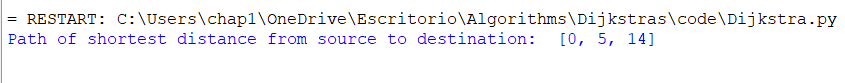
\includegraphics[scale=0.85]{results_d.png}
    \caption{Camino más corto entre 0 y 14}
    \label{fig:dijkstra}
\end{figure}
\vspace{5mm} %5mm vertical space

Se presenta arriba el codigo para obtener el camino más corto entre el vertice 0 al vertice 14, se utiliza una matriz de adjacencia. \newline
El camino más corto es 0 - 5 - 14 con un peso de 13.
\vspace{5mm} %5mm vertical space

\begin{figure}[ht]
    \centering
    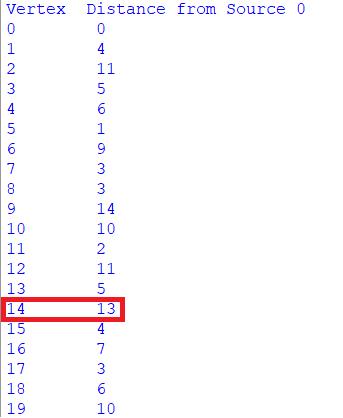
\includegraphics[scale=0.85]{wights.png}
    \caption{Camino más corto entre 0 y v}
    \label{fig:dijkstra_weights}
\end{figure}
\vspace{5mm} %5mm vertical space

\href{https://github.com/enganthony18/Algorithms}{\includegraphics[scale=0.9]{Git_link.png}}

\end{document}
